\section{Pre-Concentration System Hardware}
\subsection{Adsorbent Trap}

An adsorbent trap is a gas line filled with adsorbent material that captures and concentrates target gas species from a sample passed over it; see \figref{fig:ads trap cross section}. The trap is kept at a cold temperature (-30 °C) during sampling. The lower the trap temperature, the more capable the trap is at capturing more volatile gases. These gases are then rapidly desorbed by flash heating the trap to temperatures of 300 °C. The volatilized gas is transferred to an analysis system.

This section details the assembly of an adsorbent trap. Refer to GC operations for use of the trap.

\begin{figure}[H]
    \centering
    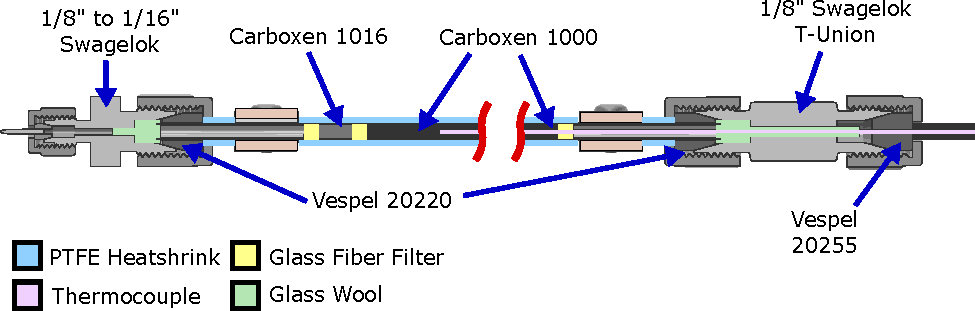
\includegraphics{Figures/microTrap Cross Section.pdf}
    \caption{Cross-section of a fully assembled adsorbent trap.}
    \label{fig:ads trap cross section}
\end{figure}

\subsubsection{Micro Trap Assembly - Materials and Equipment}
\begin{table}[H]
    \centering
    \caption{Materials required for constructing a single micro-trap.}
    \begin{tabular}{l|c|c}
        Item & P/N & Qty\\
        \hline
        1/8'' Swagelok T-union & SS-200-3 & 1\\
        Omega thermocouple & SCASS-020U-6 & 1\\
        Adsorbent & Carboxen 1000 & 200 mg\\
        Adsorbent & Graphsphere 2016 & 20 mg\\
        0.11'' OD, 0.1'' ID SS Tubing & HTX 12X-60 & 25 cm\\
        0.095'' OD, 0.067'' SS Tubing & HTX 13T-60 & 3, 5 cm\\
        Vespel reducing ferrule, drilled to 0.109 in OD & 20220 VG-2 & 2\\
        Vespel ferrule (for TC) & 20255 VG-2 & 1\\
        Millipore Glass fibre prefilter & APFD09050 & n/a\\
        \href{https://www.mcmaster.com/4864N22/}{PTFE heat shrink} & 4864N22 & 25 cm\\
        Black heat shrink & n/a & 2.5cm\\
        Glass Wool & n/a & n/a\\
    \end{tabular}
    \label{tab:ads trap materials}
\end{table}

\begin{table}[H]
    \caption{Equipment required for the construction of a micro-trap.}
    \begin{multicols}{2}
        \begin{itemize}
            \itemsep0em
            \item 100 sccm MFC (e.g., Tylan 2900 series)
            \item Diaphragm vacuum pump
            \item Rough Vacuum Gauge
            \item Stainless Steel tube cutter (e.g., Diamond cut-off saw)
            \item Scale accurate to $<$1 mg
            \item Aluminum foil
            \item Helping hands
            \item 1/4'' to 1/4'' NPT to Swagelok fitting
            \item Small aluminum tray with spout
            \item Razor knife
            \item Calipers
            \item Nitrile gloves (or equivalent)
        \end{itemize}
    \end{multicols}
    \label{tab:adsorbent trap construction equipment}
\end{table}

\subsubsection{Micro Trap Assembly - Assembly Instructions}
Place a large sheet of aluminum foil on top to create a workspace. This can be improved by placing it on an ESD mat. Carboxen is easily charged and may stick to various surfaces if handled in an electrically isolated area.
\begin{enumerate}
%\itemsep2em
\item Cut two 1/2'' pieces of black heat shrink to go over the thermocouple. Shrink them on top of each other, one at a time. This needs to build up enough thickness so that the heat shrink on the thermocouple fits snug within a 1/16'' Swagelok fitting.

\item Place 1/8'' Swagelok nut on thermocouple (threads facing away from electrical connector). Then place a 0.8 mm ID vespel ferrule on the thermocouple. Attach the thermocouple to the T-union with the heat shrink butted up against the electrical connector and the vespel ferrule.

\item Pack the side of the T-union that the thermocouple exits with glass wool. Ensure there is enough to prevent the adsorbent tubing from making an electrical connection with the union, and not too much to interfere with creating a vacuum seal. Pack it with spare tubing and remove any excess.

\item Prepare PTFE heat shrink for microtrap. Cut to 200 mm, expecting shrinkage along the length. The final length should be approximately 140 mm length after shrinking. Cut the heat shrink to length with a razor after it has been shrunk.

\item Place glass filter on the work bench with the soft side up. Insert a spare tube into the microtrap tubing; this will help keep the glass filters flush later. Press the adsorbent tube into the glass filter and roll it around on the edges to shear a piece of the glass filter that fits into the adsorbent trap tubing.

\item Flip the glass filter sheet upside-down and repeat the previous step twice to have 3 sets of glass filters inserted into the microtrap tube. Then insert a retaining tube into the microtrap and press against the spare rod until the retaining rod is flush with the microtrap tubing. Pull out the retaining tube and use a pair of pliers to slightly deform the end. Then firmly press it unto the microtrap tubing until it is flush. It should be locked in place.

\item Turn on pump and MFC. Set the MFC to 50 sccm. Vent to air to verify the MFC controller is operating. Close the valve between the gauge and where the adsorbent trap will be attached to create a vacuum and verify the pump reaches its ultimate pressure. Turn off the pump and attach it to the adsorbent trap. Turn on the pump and record the pressure. Should be roughly -1 to -3 inHg.

\item Place the 1/4'' Swagelok to 1/4'' NPT adapter on the top of the adsorbent trap. Begin slowly filling the trap with Carboxen 1000. Tap the trap housing as Carboxen is added to help it settle. Once all of the Carboxen has been added, record the vacuum. Should be roughly -3.7 to -4.4 inHg vacuum. Remove the adapter and blow out any residual Carboxen 1000. Turn off the pump to use calipers to measure the distance from the top of the tube to the bottom of the inside. There should be 2.07'' to 2.11'' remaining.

\textbf{Note:} Always have the pump off for measuring the length remaining. Then always have the pump on while adding Carboxen to help it settle.

\item Repeat the previous process but for the Carboxen 1016. Vacuum should measure between -4.1 and -4.6 inHg, and there should be 1.74 to 1.76 in left.

\item Shut off pump prior to this next step. Remove the funnel and press in 3 glass filters, soft side down on the first filter, and soft side up on the following two. Use a small spare tube to press the glass filter against the Carboxen. Turn the pump back on and measure the pressure. Should measure between -5.1 and -5.6 inHg, and the remaining length should be between 1.65'' to 1.68''.

\item Cut a retaining tube to the length you measured in the previous step using the diamond cut-off saw. File the cut down to ensure it is smooth. Use pliers to crimp one end. Push the retainer into the microtrap with the crimped side out. Measure the pressure drop again; should be between -5.4 and -5.8 inHg.

\item Install a small piece of pre-shrunk PTFE heat-shrink on the microtrap. Place a Swagelok nut and a pre-drilled ferrule on the microtrap. Fasten a plug onto the end of the trap. Vacuum the microtrap and make sure it is leak-tight.

\item Remove microtrap from vacuum line and seal the port. The trap should be sealed and ready for storage.

\end{enumerate}

\subsubsection{Adsorbent Trap Assembly}
\begin{table}[H]
    \centering
    \caption{Materials required to assemble adsorbent trap.}
    \begin{tabular}{l|c|c}
        Item & P/N & Qty\\
        \hline
        Microtrap & n/a & 1\\
        heat transfer blocks & n/a & 2\\
        Low-Power TEC,  40x40 mm, 6 A& 12706 & 2\\
        High-Power TEC, 40x40 mm, 15 A & 12715 & 2\\
        CPU Water Cooler kit & n/a & 2\\
        40 A DC Solid State Relay (SSR) & D1D40 & 1\\
        12 V, 2 A Lithium-Ion battery charger & n/a & 1\\
        3S6P 12 V Li-Ion Battery & n/a & 1\\
        Omega PID Controller & CNi16D54-32 & 1\\
        Voltage to PWM Module & n/a & 1\\
        Arctic Silver 5 Thermal Paste & AS5-3.5g & 1\\
        3D printed mounting hardware & n/a & n/a\\
        6-32 x 1/2 in Screws & n/a & 4\\
        6-32 x 1.25 in Hex Screws & n/a & 8\\
    \end{tabular}
    \label{tab: ads trap assembly materials}
\end{table}


\begin{enumerate}
\item Prepare the screw mounts on the clam shell.
    
\item Place a heat block in the clam shell, put the adsorbent trap into the block, and cover with the other half of the heat block. Make sure that the chamfered side of the clam shell is on the same side as the thermocouple.
    
\item Snap the other side of the clam shell onto the assembly. Make sure the chamfered sides of each clam shell are on the thermocouple side of the adsorbent trap.
    
\item Place the clam shell assembly on the mounting bracket and screw into place. Add the top half of the bracket and screw into place.
    
\item Place 5 dots of thermal compound on the copper block and spread as thin as possible with a small plastic spatula (typically provided with the coolers).
    
\item Place the low-power TEC on the copper block with the hot side facing away from the trap. Move laterally across the copper block to spread thermal compound. Once complete, the surface tension of the compound should hold the TEC in place.
    
\item Spread thermal compound on the hot side of the low-power TEC using the same technique that was used for the copper block.
    
\item Install a high-power TEC on top of the low-power TEC. Once again moving the TEC laterally to ensure the thermal compound is well spread.
    
\item Spread thermal compound on the hot side of the high-power TEC.
    
\item Remove any protective film from the copper block of the water cooler and place on the TEC, again moving the block laterally to help spread the thermal compound between the two surfaces. Loosely install spring-loaded screws on the mounting fins of the water cooler.
    
\item Inspect the TECs and cold block to ensure they are aligned with each other. Gently slide them into place as needed. Do the same for the water cooler and tighten into place.
    
\item Repeat the previous steps for the other side to install the 2nd TEC stack and water cooler. Keep in mind the hot side of the TEC faces towards the water cooler, so the wire colors will be flipped, not mirrored.
    
\item Attach the high-power TECs in series with the 12 V supply. Do the same for the low-power TECs. Each device will receive approximately 6 V this way.

\item Connect the PID as shown in (the schematic). Turn it on to check that it is measuring the trap temperature.

\item Connect the output of the pwm modulator to the input side of the SSR (GND to pin 4, + to pin 3). Power on the PID and set it to a low enough set point (e.g., -99 °C) and check with a voltmeter than the output power is disabled.

\item Attach the lithium-ion battery positive terminal to the positive terminal (pin 2). Check with a voltmeter that you do not measure a voltage between the negative terminal of the battery and pin 1 of the SSR. \textbf{Warning:} Connecting the wrong side of the battery to the SSR output can create a short circuit which may damage the trap. With unregulated current, this may cause the trap to overheat.

\item Remove one screw for each electrical contact on the micro-trap. Attach the negative battery terminal to one side, and pin 1 of the SSR to the other. If at any point you see a spark or observe the trap temperature spike, discontinue installation and check the SSR connections.

\item Turn on the cooler and wait up to 15 minutes to ensure the trap comes down to temperature. Note that thermal paste can take time to cure, so it may take a day or two before the trap is able to reach it's lowest temperature.

\item If the PID has previously been tuned for a micro-trap, run the sequence \say{check trap} (refer to command line operations) to verify functionality. Otherwise, you will need to tune the PID (instructions not available ATM).

\end{enumerate}

\subsection{Temperature Controller}



\subsection{Mass Flow Controllers}
\label{Mass Flow Controller}

Mass flow controllers (MFCs) are a type of specialized value that control the conduction of a valve to regulate the rate at which gas passes through the device. The successful operation of MFCs is critical to a gas sampling system as it allows for precise control of how much gas cycles through a trap. 

MFCs measure gas flow via thermal conduction. A portion of the gas stream is redirected through a heated filament and flows to an unheated filament before returning to the main gas stream. Energy transferred to the unheated filament is converted to a voltage. The MFC compares this voltage to the input set point and uses an electrical solenoid to alter how much conduction there is at the outlet of the device.

A simple analog MFC has a positive and negative supply for operating the control circuitry, an input pin for the desired set point, and an output for monitoring the flow rate. The MFC will change the flow rate as much as it can until the monitor voltage matches the set point. Since flow rate is a pressure dependent process, the inlet pressure much be large enough for the MFC to be able to achieve the desired flow rate.

The MFCs used in the pre-concentration system are off the shelf Omega Engineering devices that are controlled by a custom made control board. The MFC control board is connect to the $\pm$ 12 V, and 5 V power from the computer power supply, and a USB port from the main control board. Note that MFCs typically operate with $\pm$ 15 V. Using a lower voltage power supply for this application limits the output range to 80\%. 

The MFC control board is programmed to an ESP8266 device using microPython. Set points are controlled with a 12-bit DAC, and monitor voltages are read using a 15 bit ADC converter. This MFC control board is then connected to MFCs using a DB9 connector. See \figref{fig: MFC electronics} for a complete schematic of the MFC control board.

\subsubsection{Calibration}
Thermal transfer is a gas species dependent process. MFCs are labeled with which gas species they are calibrated for, what the maximum inlet pressure can be, and what range they can achieve (e.g., 0 - 1000 sccm). The range listed on the MFC map to a set point voltage typically ranging from 0.2 - 5.0 V. For precisely setting the flow rate on an MFC, the mapping between voltage and flow rate needs to be calibrated. The steps prescribed for using software to calibrate an MFC using the mfc.py module is described below.

\begin{enumerate}
    \item Connect MFC to the header board and open any software that connects to the header board (e.g., Thonny + USB cable).
    \item Attach pure gas to inlet of MFC (e.g., N\2, H\2, or Air). There should be greater than 40 psig on the inlet to calibrate the entire range.
    \item Attach a flow meter to the outlet of the MFC.
    \subitem Flow meter can be attached to the vent outlet on the NMHC pre-concentration system.
    \item The MFC needs to be adjusted and measured at many different flow rates to obtain an accurate calibration. Plan which set points will be used for calibration. Ideally these points will span the entire range and have multiple points near typical operating conditions. This list should contain at least 10 entries.
    \item Set the MFC to one of the calibration points and wait for the meter to stabilize. Record the set point used, and the measured flow rate.
    \item Repeat the previous step for all calibration points.
    \item Convert the set point data to raw voltage. This can be done in software using the \texttt{convert} function in calibration (e.g., \code{mfc.cal.convert(x)}). Save the voltage values as a \texttt{list}.
    \item Save the flow rate data as a \texttt{list}.
    \item Rename or otherwise archive the previous calibration file, and create a variable with the desired filename.
    \item Call \code{mfc.calibration(input\_val=[flow\_rate\_data], output\_val=[voltage], calfile=file\_name)} to run the calibration algorithm.
\end{enumerate}

\textbf{Important Calibration Considerations!}\\
Due to the digitization of the MFC signal, actual flow rates are step size limited! Converting a flow rate to an analog voltage is limited by the precision of the converter. This system uses a 12-bit digital to analog converter for a 0 - 5 V range, which yields a 1.22 mV per step resolution. For a mass flow controller with a range of 0 - 1000 sccm, this corresponds to a resolution of 0.244 sccm per step. The MFC controller checks that the output is within plus or minus 1.5 steps. For example, a 0 - 1000 sccm controller's range corresponds to 0.2 - 5 V. Requesting the controller set the flow rate to 50 sccm will set an output voltage that corresponds to 49.9 sccm. The controller then only verifies the output stabilizes within the range of 49.5 - 50.3 sccm. A larger potential error for operators is ignoring the limitations of the mass flow controller. The system does not error if an excessively large value is called. The flow controller handles this by simply setting the output to be fully on and not checking the output. For example \code{sample(1000)} will set the controller to output a signal that corresponds to a 200 sccm flow rate.
\pagebreak